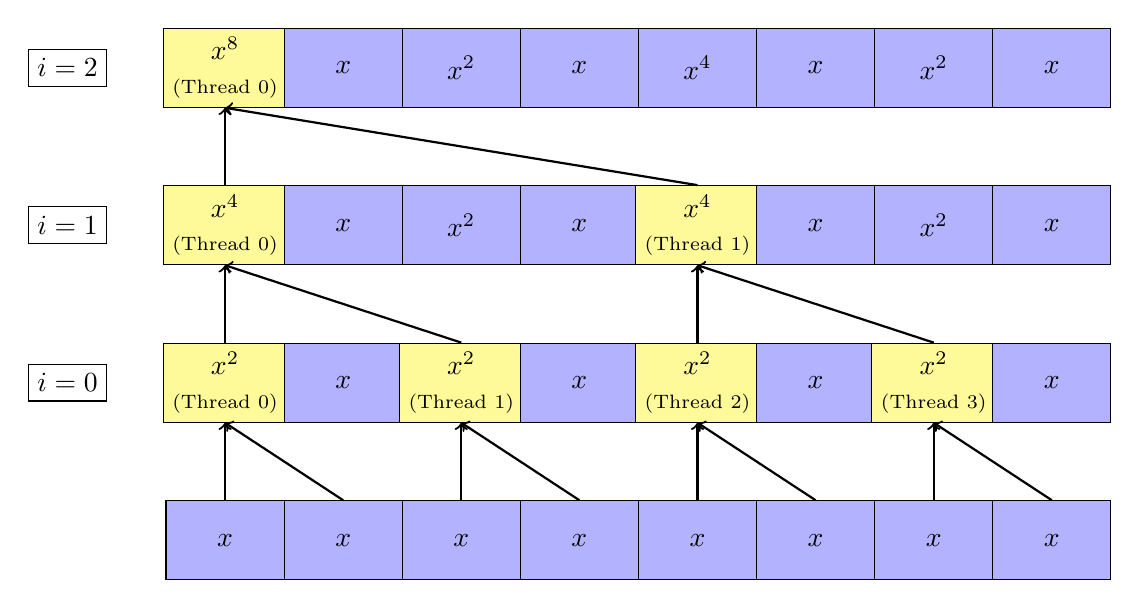
\begin{tikzpicture}[level/.style={sibling distance=60mm/#1}]

\def\HEIGHT{1}
\def\WIDTH{1.5}

% leaves
\node (rect) at (0*\WIDTH,0) [draw,minimum width=\WIDTH cm,minimum height=\HEIGHT cm, fill=blue!30] (a0) {$x$};
\node (rect) at (1*\WIDTH,0) [draw,minimum width=\WIDTH cm,minimum height=\HEIGHT cm, fill=blue!30] (a1) {$x$};
\node (rect) at (2*\WIDTH,0) [draw,minimum width=\WIDTH cm,minimum height=\HEIGHT cm, fill=blue!30] (a2) {$x$};
\node (rect) at (3*\WIDTH,0) [draw,minimum width=\WIDTH cm,minimum height=\HEIGHT cm, fill=blue!30] (a3) {$x$};
\node (rect) at (4*\WIDTH,0) [draw,minimum width=\WIDTH cm,minimum height=\HEIGHT cm, fill=blue!30] (a4) {$x$};
\node (rect) at (5*\WIDTH,0) [draw,minimum width=\WIDTH cm,minimum height=\HEIGHT cm, fill=blue!30] (a5) {$x$};
\node (rect) at (6*\WIDTH,0) [draw,minimum width=\WIDTH cm,minimum height=\HEIGHT cm, fill=blue!30] (a6) {$x$};
\node (rect) at (7*\WIDTH,0) [draw,minimum width=\WIDTH cm,minimum height=\HEIGHT cm, fill=blue!30] (a7) {$x$};

\node (rect) at (0*\WIDTH,2) [draw,minimum width=\WIDTH cm,minimum height=\HEIGHT cm, fill=yellow!40, align=center] (b0) {$x^2$\\\scriptsize{(Thread 0)}};
\node (rect) at (1*\WIDTH,2) [draw,minimum width=\WIDTH cm,minimum height=\HEIGHT cm, fill=blue!30] (b1) {$x$};
\node (rect) at (2*\WIDTH,2) [draw,minimum width=\WIDTH cm,minimum height=\HEIGHT cm, fill=yellow!40, align=center] (b2) {$x^2$\\\scriptsize{(Thread 1)}};
\node (rect) at (3*\WIDTH,2) [draw,minimum width=\WIDTH cm,minimum height=\HEIGHT cm, fill=blue!30] (b3) {$x$};
\node (rect) at (4*\WIDTH,2) [draw,minimum width=\WIDTH cm,minimum height=\HEIGHT cm, fill=yellow!40, align=center] (b4) {$x^2$\\\scriptsize{(Thread 2)}};
\node (rect) at (5*\WIDTH,2) [draw,minimum width=\WIDTH cm,minimum height=\HEIGHT cm, fill=blue!30] (b5) {$x$};
\node (rect) at (6*\WIDTH,2) [draw,minimum width=\WIDTH cm,minimum height=\HEIGHT cm, fill=yellow!40, align=center] (b6) {$x^2$\\\scriptsize{(Thread 3)}};
\node (rect) at (7*\WIDTH,2) [draw,minimum width=\WIDTH cm,minimum height=\HEIGHT cm, fill=blue!30] (b7) {$x$};

\node (rect) at (0*\WIDTH,4) [draw,minimum width=\WIDTH cm,minimum height=\HEIGHT cm, fill=yellow!40, align=center] (c0) {$x^4$\\\scriptsize{(Thread 0)}};
\node (rect) at (1*\WIDTH,4) [draw,minimum width=\WIDTH cm,minimum height=\HEIGHT cm, fill=blue!30] (c1) {$x$};
\node (rect) at (2*\WIDTH,4) [draw,minimum width=\WIDTH cm,minimum height=\HEIGHT cm, fill=blue!30] (c2) {$x^2$};
\node (rect) at (3*\WIDTH,4) [draw,minimum width=\WIDTH cm,minimum height=\HEIGHT cm, fill=blue!30] (c3) {$x$};
\node (rect) at (4*\WIDTH,4) [draw,minimum width=\WIDTH cm,minimum height=\HEIGHT cm, fill=yellow!40, align=center] (c4) {$x^4$\\\scriptsize{(Thread 1)}};
\node (rect) at (5*\WIDTH,4) [draw,minimum width=\WIDTH cm,minimum height=\HEIGHT cm, fill=blue!30] (c5) {$x$};
\node (rect) at (6*\WIDTH,4) [draw,minimum width=\WIDTH cm,minimum height=\HEIGHT cm, fill=blue!30] (c6) {$x^2$};
\node (rect) at (7*\WIDTH,4) [draw,minimum width=\WIDTH cm,minimum height=\HEIGHT cm, fill=blue!30] (c7) {$x$};

\node (rect) at (0*\WIDTH,6) [draw,minimum width=\WIDTH cm,minimum height=\HEIGHT cm, fill=yellow!40, align=center] (d0) {$x^8$\\\scriptsize{(Thread 0)}};
\node (rect) at (1*\WIDTH,6) [draw,minimum width=\WIDTH cm,minimum height=\HEIGHT cm, fill=blue!30] (d1) {$x$};
\node (rect) at (2*\WIDTH,6) [draw,minimum width=\WIDTH cm,minimum height=\HEIGHT cm, fill=blue!30] (d2) {$x^2$};
\node (rect) at (3*\WIDTH,6) [draw,minimum width=\WIDTH cm,minimum height=\HEIGHT cm, fill=blue!30] (d3) {$x$};
\node (rect) at (4*\WIDTH,6) [draw,minimum width=\WIDTH cm,minimum height=\HEIGHT cm, fill=blue!30] (d4) {$x^4$};
\node (rect) at (5*\WIDTH,6) [draw,minimum width=\WIDTH cm,minimum height=\HEIGHT cm, fill=blue!30] (d5) {$x$};
\node (rect) at (6*\WIDTH,6) [draw,minimum width=\WIDTH cm,minimum height=\HEIGHT cm, fill=blue!30] (d6) {$x^2$};
\node (rect) at (7*\WIDTH,6) [draw,minimum width=\WIDTH cm,minimum height=\HEIGHT cm, fill=blue!30] (d7) {$x$};

\node[draw] at (-2,2) {$i=0$};
\node[draw] at (-2,4) {$i=1$};
\node[draw] at (-2,6) {$i=2$};

% print paths
\draw[thick, ->] (a0.north) -- (b0.south);
\draw[thick, ->] (a1.north) -- (b0.south);
\draw[thick, ->] (a2.north) -- (b2.south);
\draw[thick, ->] (a3.north) -- (b2.south);
\draw[thick, ->] (a4.north) -- (b4.south);
\draw[thick, ->] (a5.north) -- (b4.south);
\draw[thick, ->] (a6.north) -- (b6.south);
\draw[thick, ->] (a7.north) -- (b6.south);

\draw[thick, ->] (b0.north) -- (c0.south);
\draw[thick, ->] (b2.north) -- (c0.south);
\draw[thick, ->] (b4.north) -- (c4.south);
\draw[thick, ->] (b6.north) -- (c4.south);

\draw[thick, ->] (c0.north) -- (d0.south);
\draw[thick, ->] (c4.north) -- (d0.south);

\end{tikzpicture}